A peephole optimiser rewrites assembly code to make ik more efficient, in terms of processor cycles and memory usage. The general procedure is:
\begin{enumerate}
\item assembly parsing;
\item division in basic blocks;
\item optimisation;
\item assembly generation.
\end{enumerate}
See also figure~\ref{fig:diagram}. We discuss stages 1 and 4 first and then stage 2 and stage 3.

\begin{figure}[h!]
\centering
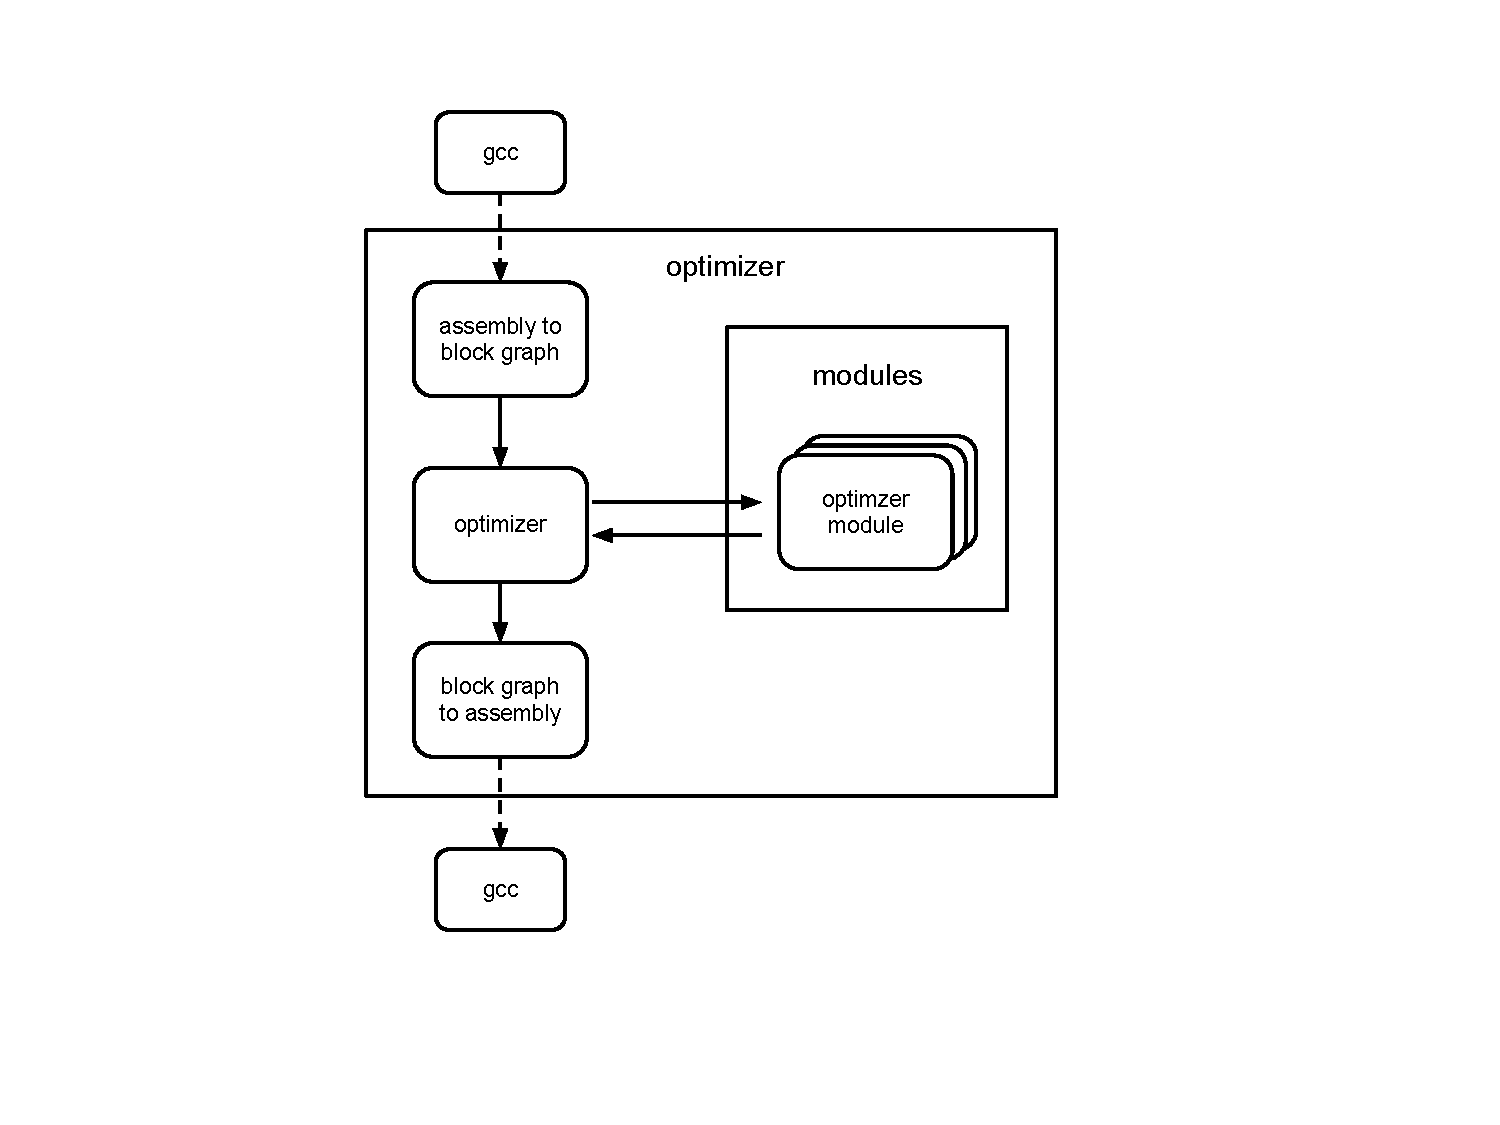
\includegraphics[viewport= 170 90 510 490, clip=true]{diagram}
\caption{Optimiser design diagram.}
\label{fig:diagram}
\end{figure}


\subsection*{Assembly parsing and generation}
As processing an assembly program in the form of a set of text strings is difficult, the optimiser translates the input to an intermediate representation (ir) in the first stage. This translation is called \emph{parsing}. The resulting representation is a list of Python objects, where each object represents an assembly instruction. After optimising, the resulting intermediate representation is translated back to assembly code. Ideally, when no optimisation is done between parsing assembly and regenerating assembly, the composite function $4\circ 1$ is the identity function on the set of all assembly programs. (In our implementation, comments are left out in some cases, and spacing is sometimes changed.)

\subsection*{Division in basic blocks}
Before optimising, the ir is split in \emph{basic blocks}. A basic block is a set of consecutive instructions having a single entry point and a single exit point. By definition, only the first line $i_1$ of a basic block $(i_1, \ldots, i_k)$ can be a jump destination and only the last line $i_k$ can be a jump. Therefore, the execution flow is always $i_1\rightarrow i_2 \rightarrow \cdots \rightarrow i_k$. This property reduces the complexity of doing certain optimisations on instructions in a basic block.

Basic blocks can in turn be divided in functions, linked together by \emph{jump and link} instructions, \code{jal}. We call the set of instructions in a function a \emph{frame}. Frames have a single entry point (on frame level), but not necessarily a single exit point.

\subsection*{Optimisation}
In the optimisation stage, the original intermediate representation $A$ is transformed into a new ir $B$, such that
\begin{enumerate}
\item the new representation $B$ has the same \emph{meaning} as $A$, in terms of program output and behaviour;
\item the execution of the program corresponding to $B$ takes less processor cycles and uses less memory.
\end{enumerate}

\subsubsection*{Optimisation types}
There are two main types of optimisations: graph level optimisations and block level optimisations. 
Our optimiser performs the following graph optimisations:
\begin{itemize}
\item unused block removal,
\item graph flattening, and
\item global branch optimisations,
\end{itemize}
and the following block optimisations:
\begin{itemize}
\item dead code elimination,
\item copy propagation, and
\item constant folding.
\end{itemize}
The optimisations are explained in the implementation sections that follow.


\subsubsection*{Scheduling}
As there are multiple optimisations to apply and a single optimisation may be applied multiple times, we must decide how to schedule them. In this sections we will regard graph and block optimisations as functions on the set of control flow graphs and ir blocks, respectively.

Let $f$ be an optimisation on blocks. It is possible that an application of $f$ on a block $B$ yields a block that in turn can be optimised. That is, applying $f$ on $f(B)$ will yield a different result than $f(B)$. Therefore, $f$ is applied to $B$ until the result is constant, i.e. $n$ times, with $$f^{(n)}(B) = f^{(n-1)}(B).$$ We denote the function that applies $f$ until the result is stable by $f^*$. Note that $f^{(k)}(B)$ for some $k$ need not necessarily be more efficient than $B$ to be useful, because other optimisations can take advantage of the changes made. For example, copy propagation only pays off after dead code elimination.

Let $f$ and $g$ be two different optimisations on blocks. We could apply $f^*$ to a block $B$ and then $g^*$. But, as $f^*$ and $g^*$ may be mutually beneficial, the composite application $g^* \circ f^*$ must be repeated until the result is constant.

The same properties hold when $f$ and $g$ are graph level optimisations, \emph{mutatis mutandis}. We could even mix graph and block optimisations, where block optimisations are applied to all blocks in the graph concerned. Let $F_1, \ldots, F_m$ be such optimisations. Then, every optimisation must be repeated until constant, which we called $F_i^*$, and the composite optimisation must also be repeated until constant, giving $${(F_m^* \circ \cdots \circ F_1^*)}^*.$$ This is the general scheduling recipe.

We did not consider the order of applying optimisations. A particular order could be optimal. However, as the composite optimisation is repeated until the result is constant, the precise order probably is not decisive.
\newline
In the following sections we will look at the implementation of the four stages


